\subsection{OB-4 (APS)}
Instrukční cyklus počítače a zřetězené zpracování instrukcí. Mikroarchitektura skalárního procesoru se zře\-tě\-ze\-ným zpracováním instrukcí, datové a řídicí hazardy při zřetězeném zpracování instrukcí a způsoby jejich ošetření.

\textbf{Definice 1:}
ISA (Instruction Set Architecture) je abstraktní rozhraní mezi HW a nízkoúrovňovým SW, které zahrnuje vše nezbytné pro psaní korektních programů ve strojovém jazyce. Zahrnuje instrukční sadu, registry, organizaci paměti, vstupy a výstupy,...

\textbf{Definice 2:}
ISA je kompletní instrukční sada procesoru, včetně adresních módů.

\textbf{Mikroarchitektura:}
Mikroarchitektura je detailní interní organizace procesoru, včetně hlavních
funkčních jednotek, jejich propojení a řízení.

\subsubsection*{Instrukční cyklus počítače}
\begin{itemize}
	\item IF --- Instruction Fetch
	\item ID/OF --- Instruction Decode and Operand Fetch
	\item EX --- Execute
	\item MEM --- Memory access
	\item WB --- Write Back
\end{itemize}

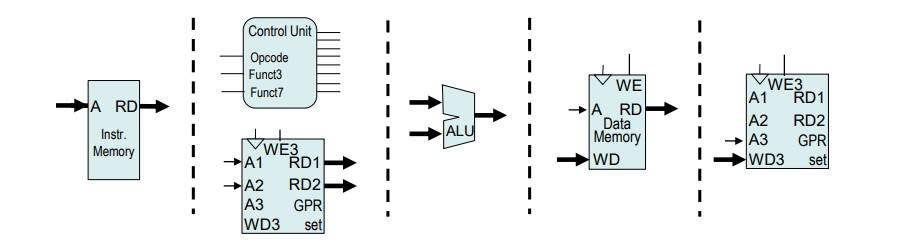
\includegraphics[width=0.8\textwidth]{img/OB-4_0.jpg}

\subsubsection*{Zřetězené zpracování instrukcí}
Instrukce se dle svých fází rozdělí a v procesoru vykonává postupně. Procesor je rozdělen dělícími registry. Instrukce se zpracovává postupně v rozdělených částech procesoru, vykonává se zároveň více instrukcí naráz (v různých fázích).



\subsubsection*{Mikroarchitektura skalárního procesoru se zřetězeným zpracováním instrukcí}

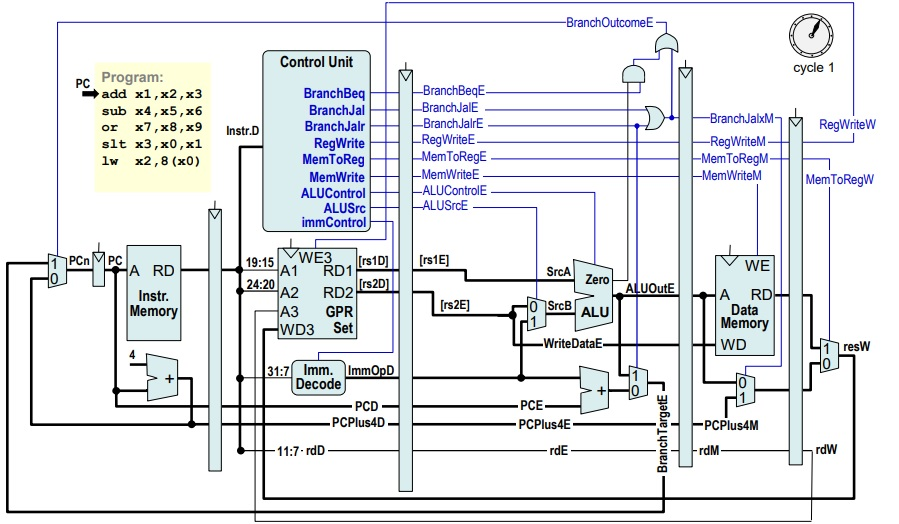
\includegraphics[width=0.9\textwidth]{img/OB-4_1.jpg}

\subsubsection*{Hazardy}
Protože je rozpracováno více instrukcí najednou, mohou vznikat konflikty při
přístupu ke sdíleným prostředkům počítače. Tomu se říká hazardy.
Sdíleným prostředkem je prostředek, který je opakovaně použit v různých
stupních instrukčního zřetězení.

Typy hazardů:
\begin{itemize}
	\item datové (důsledek datových závislostí: RAW, WAR, WAW)
	\item řídící (instrukce měnící PC, tedy obsah fronty instrukcí)
	\item strukturální (počet současných požadavků na daný prostředek převyšuje počet jeho instancí)
\end{itemize}

Hazardy mohou způsobovat pozastavení instrukčního zřetězení (stall) nebo vyprázdnění (flush).

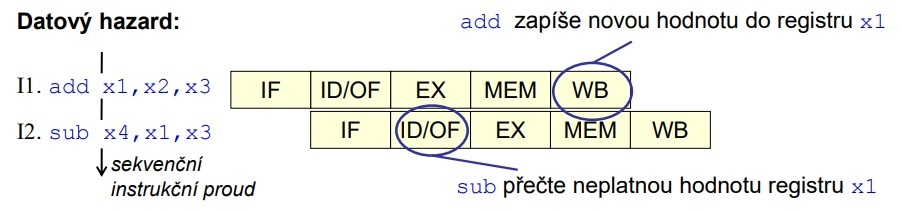
\includegraphics[width=0.8\textwidth]{img/OB-4_2.jpg}

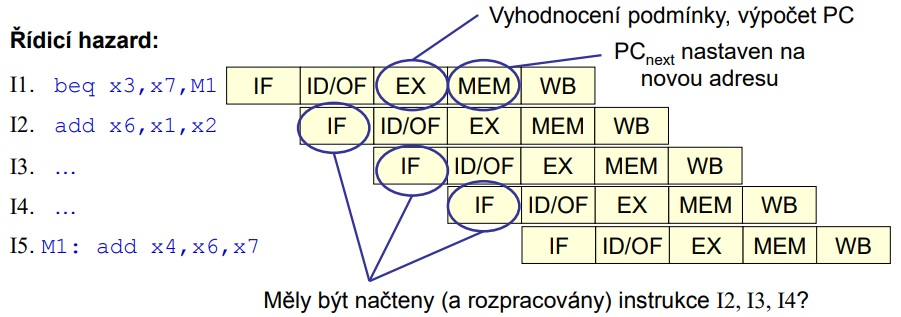
\includegraphics[width=0.8\textwidth]{img/OB-4_3.jpg}

Možnosti řešení hazardů:
\begin{itemize}
	\item přeposílání (forwarding)
	
	Lze použít v případě datového hazardu, kdy výsledek předchozí instrukce požadovaný instrukcí nasledující vznikne dříve nebo ve stejném cyklu, kdy má být následující instrukcí použit. Výsledek je přeposlán tam, kde je potřeba (část EX). 	
	
	\item pozastavení (stall)
	
	Lze použít v případě datového hazardu, kdy je výsledek předchozí instrukce potřeba před jeho vznikem. Zpracovávání následujících instrukcí se pozastaví a vyplní se instrukce nop (bublina). V dalších instrukcích se pokračuje, když výsledek existuje --- lze jej tedy přeposlat.	
	
	Také může řešit strukturální hazardy.
	
	\item vyprázdnění části pipeline (flush)
	
	Lze použít v řídících hazardech, kdy se PC nastaví na neočekávanou adresu nějakou skokovou instrukcí. Všechny již načtené a zpracovávané instrukce, které následují po skoku, se musí z fronty odstranit, a následuje zpracovávání instrukcí z chtěné adresy (kam skok skočil).
\end{itemize}

Hazardy řeší nová jednotka v procesoru --- HMU (Hazard Management Unit).
